% !TeX program = xelatex
\documentclass[a4paper,10pt]{article}

% ============================================================================
% សន្លឹកកិច្ចការសិស្ស ស-ខ្មៅ (Student Guided-Inquiry Worksheet - Grade 8 15.2.2 CIRC4)
% បរិបទ៖ ថ្នាក់រៀនគ្មានស្លាយ LCD – រុករកលក្ខណៈឆ្លុះនៃរង្វង់ដោយបន្ទាត់ក្រិត និងអេគែរ ២ ទំព័រ A4
% ============================================================================
\usepackage[a4paper, left=0.90cm, right=0.90cm, top=0.75cm, bottom=0.85cm, footskip=0.45cm]{geometry}
\usepackage{amsmath, amssymb}
\usepackage{unicode-math}
\usepackage{fontspec}
\usepackage{array, colortbl}
\usepackage[table]{xcolor}
\usepackage{enumitem}
\usepackage{pifont}
\usepackage{fancyhdr}
\usepackage{lastpage}
\usepackage{tikz}
\usepackage[most]{tcolorbox}
\usetikzlibrary{calc, arrows.meta, angles, quotes, decorations.markings, positioning, babel}

\makeatletter
\let\@expl@@@mark@update@singlecol@structures@@\relax
\makeatother

\providecommand{\NGSFindFonts}{%
  \IfFileExists{C:/Windows/Fonts/cambria.ttc}{%
    \def\NGSSysPath{C:/Windows/Fonts/}%
    \def\NGSUserPath{C:/Users/KIT/AppData/Local/Microsoft/Windows/Fonts/}%
  }{%
    \IfFileExists{./fonts/KhmerOSsiemreap.ttf}{\def\NGSSysPath{./fonts/}\def\NGSUserPath{./fonts/}}{%
    \IfFileExists{../fonts/KhmerOSsiemreap.ttf}{\def\NGSSysPath{../fonts/}\def\NGSUserPath{../fonts/}}{%
    \IfFileExists{../../fonts/KhmerOSsiemreap.ttf}{\def\NGSSysPath{../../fonts/}\def\NGSUserPath{../../fonts/}}{%
    \IfFileExists{../../../fonts/KhmerOSsiemreap.ttf}{\def\NGSSysPath{../../../fonts/}\def\NGSUserPath{../../../fonts/}}{%
    \IfFileExists{../../../../fonts/KhmerOSsiemreap.ttf}{\def\NGSSysPath{../../../../fonts/}\def\NGSUserPath{../../../../fonts/}}{%
    \IfFileExists{../../../../../fonts/KhmerOSsiemreap.ttf}{\def\NGSSysPath{../../../../../fonts/}\def\NGSUserPath{../../../../../fonts/}}{%
    \IfFileExists{../../../../../../fonts/KhmerOSsiemreap.ttf}{\def\NGSSysPath{../../../../../../fonts/}\def\NGSUserPath{../../../../../../fonts/}}{%
      \def\NGSSysPath{../../../../../../../fonts/}\def\NGSUserPath{../../../../../../../fonts/}%
    }}}}}}}%
  }%
}
\NGSFindFonts

\setmathfont[Path={\NGSSysPath}, FontIndex=1, Scale=1.02]{cambria.ttc}
\defaultfontfeatures{Ligatures=TeX}

\setmainfont[
  Path={\NGSUserPath},
  Extension=.ttf,
  Script=Khmer,
  BoldFont={KhmerOSsiemreap},
  BoldFeatures={FakeBold=1.8},
  ItalicFont={KhmerOSsiemreap},
  ItalicFeatures={FakeSlant=0.25},
  BoldItalicFont={KhmerOSsiemreap},
  BoldItalicFeatures={FakeBold=1.8, FakeSlant=0.25}
]{KhmerOSsiemreap}

\newfontfamily\muol[Path={\NGSUserPath}, Extension=.ttf, Script=Khmer]{KhmerOSmuollight}
\newfontfamily\TimesEn[Path={\NGSSysPath}, Extension=.ttf, BoldFont={timesbd}, ItalicFont={timesi}, BoldItalicFont={timesbi}]{times}

\XeTeXlinebreaklocale "km"
\XeTeXlinebreakskip = 0pt plus 1pt minus 0.1pt

\definecolor{panelgray}{gray}{0.94}
\definecolor{headgray}{gray}{0.86}

\pagestyle{fancy}
\fancyhf{}
\renewcommand{\headrulewidth}{0pt}
\fancyfoot[L]{\fontsize{8pt}{10pt}\selectfont អនុវិទ្យាល័យព្រះក្រសាំង \en{|} គណិតវិទ្យា ថ្នាក់ទី៨ \en{|} មេរៀនទី១៥ (២.២ លក្ខណៈឆ្លុះនៃរង្វង់)}
\fancyfoot[R]{\fontsize{8.2pt}{10pt}\selectfont ទំព័រ \en{\thepage\ / \pageref{LastPage}}}

\setlength{\parindent}{0pt}
\setlength{\parskip}{0pt}
\setlength{\tabcolsep}{4pt}

\newcommand{\en}[1]{{\TimesEn #1}}
\newcommand{\enbf}[1]{{\TimesEn\textbf{#1}}}
\newcommand{\unit}[1]{\,\text{\en{#1}}}
\newcommand{\cnum}[1]{{\fontsize{10pt}{12pt}\selectfont\ding{\numexpr171+#1\relax}}}
\newcommand{\chk}{\tikz[baseline=-0.15ex]\draw[black, line width=0.8pt] (0,0) rectangle (0.25cm,0.25cm);}
\newcommand{\tri}[1]{\ensuremath{\triangle #1}}
\newcommand{\ang}[1]{\ensuremath{\angle #1}}
\newcommand{\arc}[1]{\ensuremath{\widehat{#1}}}
\newcommand{\cg}{\ensuremath{\cong}}
\newcommand{\dotline}[1]{\makebox[#1]{\dotfill}}

\newcolumntype{L}[1]{>{\raggedright\arraybackslash}p{#1}}
\newcolumntype{C}[1]{>{\centering\arraybackslash}p{#1}}

\tikzset{
  tk1/.style={postaction={decorate},decoration={markings,mark=at position 0.50 with {\draw[black, line width=0.90pt](0,-0.095)--(0,0.095);}}},
  tk2/.style={postaction={decorate},decoration={markings,
    mark=at position 0.45 with {\draw[black, line width=0.90pt](0,-0.095)--(0,0.095);},
    mark=at position 0.55 with {\draw[black, line width=0.90pt](0,-0.095)--(0,0.095);}}}
}

\newcommand{\secbar}[2]{%
  \vspace{3pt}
  \noindent\colorbox{headgray}{\parbox{\dimexpr\linewidth-2\fboxsep\relax}{%
    \vspace{1.5pt}{\muol\fontsize{9.5pt}{13.5pt}\selectfont #1}\hfill{\fontsize{8.5pt}{12pt}\selectfont\textbf{#2}}\vspace{1.5pt}%
  }}\par\vspace{3pt}
}

\begin{document}
\fontsize{9.5pt}{14.3pt}\selectfont

% ============================================================================
% ទំព័រទី១៖ ក្បាលសន្លឹកកិច្ចការ + E1 + E2 (ខ្នាតពិត 1:1) + E3
% ============================================================================
\begin{tcolorbox}[enhanced, sharp corners, colback=white, colframe=black, boxrule=1.0pt, top=4pt, bottom=4pt, left=6pt, right=6pt]
  \begin{center}
    {\muol\fontsize{10.5pt}{15pt}\selectfont សន្លឹកកិច្ចការសិស្ស — មេរៀនទី១៥៖ រង្វង់ \enbf{(}២.២ លក្ខណៈឆ្លុះនៃរង្វង់\enbf{)}}\\[2pt]
    {\footnotesize សៀវភៅសិក្សាគោលថ្នាក់ទី៨ ទំព័រ ២០២--២០៤ \en{|} រុករកដោយបន្ទាត់ក្រិត ដែកឈាន និងអេគែរ (គ្មានស្លាយ \en{LCD})}
  \end{center}
  \vspace{2pt}
  \hrule height 0.5pt
  \vspace{4pt}
  ឈ្មោះសិស្ស៖ \dotline{5.3cm} ថ្នាក់៖ \dotline{2.0cm} ដៃគូទី៖ \dotline{2.0cm} កាលបរិច្ឆេទ៖ \dotline{3.3cm}
\end{tcolorbox}

% -------------------- ផ្នែកទី១៖ E1 ENGAGE --------------------
\secbar{ផ្នែកទី១ ៖ បេសកកម្មភ្ជាប់បញ្ហា \enbf{(E1 — Engage)} — ទទឹងផ្ទៃទឹកក្នុងលូបេតុងមូល}{\en{3} នាទី (ទស្សន៍ទាយមុនរៀន)}

\begin{tcolorbox}[enhanced, sharp corners, colback=panelgray, colframe=black, boxrule=0.8pt, top=3pt, bottom=3pt, left=6pt, right=6pt]
  \begin{minipage}[c]{13.1cm}
    លូបេតុងរាងរង្វង់មួយមានកាំខាងក្នុង $OD = 5\unit{dm}$ ។ ផ្ទៃទឹកផ្ដេកបង្កើតបានជាអង្កត់ធ្នូ $CD$ ដែលស្ថិតនៅចម្ងាយកែង $OH = 3\unit{dm}$ ក្រោមផ្ចិត $O$ ($OH \perp CD$) ។ តើទទឹងផ្ទៃទឹកទាំងមូល $CD$ មានប្រវែងស្មើប៉ុន្មាន?\\[2pt]
    $\bullet$ \textbf{ការទស្សន៍ទាយដំបូងរបស់ប្អូន៖}\quad
    \chk\ មតិទី១៖ តាមពីតាករ $\sqrt{5^2-3^2}=4$ ដូច្នេះ $CD = 4\unit{dm}$\\[1.5pt]
    \hspace*{4.55cm}\chk\ មតិទី២៖ $HD = 4\unit{dm}$ ជាពាក់កណ្ដាលអង្កត់ធ្នូ ដូច្នេះ $CD = 2\times 4 = 8\unit{dm}$ \quad \chk\ មិនទាន់ប្រាកដ
  \end{minipage}\hfill
  \begin{minipage}[c]{5.2cm}
    \centering
    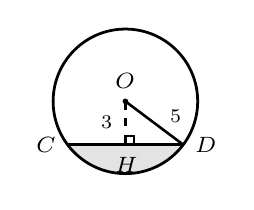
\begin{tikzpicture}[scale=0.68, every node/.style={font=\footnotesize, text=black}]
      \coordinate (O) at (2.0,1.45);
      \begin{scope}
        \clip (O) circle (1.35);
        \fill[gray!22] (0.5,0.0) rectangle (3.5,0.64);
      \end{scope}
      \draw[black, line width=1.0pt] (O) circle (1.35);
      \coordinate (C) at (0.92,0.64);
      \coordinate (D) at (3.08,0.64);
      \coordinate (H) at (2.00,0.64);
      \draw[black, line width=1.05pt] (C)--(D);
      \draw[black, line width=0.85pt, dashed] (O)--(H);
      \draw[black, line width=0.95pt] (O)--(D);
      \draw[black, line width=0.7pt] ($(H)+(0,0.16)$)--($(H)+(0.16,0.16)$)--($(H)+(0.16,0)$);
      \fill[black] (O) circle (1.5pt) node[above=1pt] {$O$};
      \node[below=1pt] at (H) {$H$};
      \node[left=1pt] at (C) {$C$};
      \node[right=1pt] at (D) {$D$};
      \node[right=2pt] at (2.55,1.18) {\scriptsize $5$};
      \node[left=1pt] at (2.00,1.05) {\scriptsize $3$};
    \end{tikzpicture}
  \end{minipage}
\end{tcolorbox}

% -------------------- ផ្នែកទី២៖ E2 EXPLORE --------------------
\secbar{ផ្នែកទី២ ៖ រុករកតាមខ្នាតពិត \enbf{1:1} និងអ័ក្សឆ្លុះអង្កត់ផ្ចិត \enbf{(E2 — Explore)}}{\en{11} នាទី (ពិភាក្សាដៃគូ)}

\begin{tcolorbox}[enhanced, sharp corners, colback=white, colframe=black, boxrule=0.85pt, top=4pt, bottom=4pt, left=6pt, right=6pt]
  \begin{minipage}[c]{9.0cm}
    \centering
    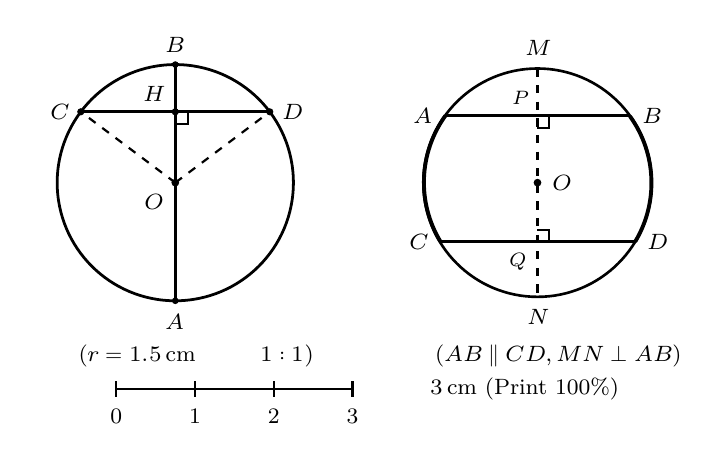
\begin{tikzpicture}[x=1cm, y=1cm, every node/.style={font=\footnotesize, text=black}]
      % រូប ក៖ រង្វង់ខ្នាតពិត 1:1 កាំ r = 1.50 cm (OH = 0.90 cm, HC = HD = 1.20 cm)
      \coordinate (O) at (1.75,2.00);
      \draw[black, line width=1.0pt] (O) circle (1.50);
      \coordinate (A) at (1.75,0.50);
      \coordinate (B) at (1.75,3.50);
      \coordinate (H) at (1.75,2.90);
      \coordinate (C) at (0.55,2.90);
      \coordinate (D) at (2.95,2.90);
      \draw[black, line width=1.0pt] (A)--(B);
      \draw[black, line width=1.05pt] (C)--(D);
      \draw[black, line width=0.80pt, dashed] (O)--(C) (O)--(D);
      \draw[black, line width=0.75pt] ($(H)+(0,-0.16)$)--($(H)+(0.16,-0.16)$)--($(H)+(0.16,0)$);
      \fill[black] (O) circle (1.4pt) node[below left=1pt] {$O$};
      \fill[black] (H) circle (1.3pt) node[above left=0.5pt] {$H$};
      \fill[black] (A) circle (1.2pt) node[below=1pt] {$A$};
      \fill[black] (B) circle (1.2pt) node[above=1pt] {$B$};
      \fill[black] (C) circle (1.3pt) node[left=1pt] {$C$};
      \fill[black] (D) circle (1.3pt) node[right=1pt] {$D$};
      \node[anchor=north] at (1.75,0.06) {\textbf{រូប ក} ($r=1.5\unit{cm}$ ខ្នាតពិត $1:1$)};

      % រូប ខ៖ អង្កត់ធ្នូស្រប AB // CD និងអង្កត់ផ្ចិតជំនួយកែង MN
      \begin{scope}[shift={(4.55,0)}]
        \coordinate (O2) at (1.80,2.00);
        \draw[black, line width=0.95pt] (O2) circle (1.45);
        \coordinate (M1) at (1.80,3.45);
        \coordinate (N1) at (1.80,0.55);
        \coordinate (A1) at (0.63,2.85);
        \coordinate (B1) at (2.97,2.85);
        \coordinate (P1) at (1.80,2.85);
        \coordinate (C1) at (0.56,1.25);
        \coordinate (D1) at (3.04,1.25);
        \coordinate (Q1) at (1.80,1.25);
        \draw[black, line width=0.90pt, dashed] (M1)--(N1);
        \draw[black, line width=1.05pt] (A1)--(B1) (C1)--(D1);
        \draw[black, line width=1.40pt] (A1) arc (144.3:211.0:1.45);
        \draw[black, line width=1.40pt] (D1) arc (-31.0:35.7:1.45);
        \draw[black, line width=0.75pt] ($(P1)+(0,-0.15)$)--($(P1)+(0.15,-0.15)$)--($(P1)+(0.15,0)$);
        \draw[black, line width=0.75pt] ($(Q1)+(0,0.15)$)--($(Q1)+(0.15,0.15)$)--($(Q1)+(0.15,0)$);
        \fill[black] (O2) circle (1.4pt) node[right=2pt] {$O$};
        \node[above=1pt] at (M1) {$M$};
        \node[below=1pt] at (N1) {$N$};
        \node[left=1pt] at (A1) {$A$};
        \node[right=1pt] at (B1) {$B$};
        \node[left=1pt] at (C1) {$C$};
        \node[right=1pt] at (D1) {$D$};
        \node[above left=0.5pt] at (P1) {\scriptsize $P$};
        \node[below left=0.5pt] at (Q1) {\scriptsize $Q$};
        \node[anchor=north] at (1.80,0.06) {\textbf{រូប ខ} ($AB\parallel CD, MN\perp AB$)};
      \end{scope}

      % បន្ទះក្រិតខ្នាតពិត 3 cm (Print 100%)
      \draw[black, line width=0.9pt] (1.00,-0.62) -- (4.00,-0.62);
      \foreach \x/\lbl in {1.00/0, 2.00/1, 3.00/2, 4.00/3} {
        \draw[black, line width=0.8pt] (\x,-0.72) -- (\x,-0.52);
        \node[below=2pt] at (\x,-0.68) {\en{\lbl}};
      }
      \node[right=4pt] at (4.00,-0.62) {\footnotesize ខ្នាតពិត $\en{3\unit{cm}}$ (\en{Print 100\%})};
    \end{tikzpicture}
  \end{minipage}\hfill
  \begin{minipage}[c]{9.2cm}
    \textbf{១. ពិនិត្យរូប ក (អង្កត់ផ្ចិត $AB \perp CD$ ត្រង់ $H$, $OH = 0.9\unit{cm}$)៖}\\[1.5pt]
    $\bullet$ ប្រើបន្ទាត់ក្រិតវាស់៖ $HC =$ \dotline{1.0cm}$\unit{cm}$ និង $HD =$ \dotline{1.0cm}$\unit{cm}$ ឯ $CD =$ \dotline{1.0cm}$\unit{cm}$ ។\\[1.5pt]
    $\bullet$ ក្នុងត្រីកោណកែង $\tri{OHC}$ និង $\tri{OHD}$ មានកាំ $OC = OD =$ \dotline{1.0cm}$\unit{cm}$ និងជ្រុងរួម \dotline{0.9cm} $\implies \tri{OHC}\cg\tri{OHD} \implies HC =$ \dotline{1.0cm} និងធ្នូ $\arc{CB} =$ \dotline{1.0cm} ។\\[1.5pt]
    $\bullet$ ផ្ទៀងតាមពីតាករ៖ $OH^2 + HD^2 = 0.9^2 + 1.2^2 =$ \dotline{1.1cm} $= 1.5^2 = OD^2$ ។\\[3pt]
    \textbf{២. ពិនិត្យរូប ខ (ធ្នូចន្លោះអង្កត់ធ្នូស្រប $AB \parallel CD$, ទំ.២០៣)៖}\\[1.5pt]
    $\bullet$ គូសអង្កត់ផ្ចិតជំនួយ $MN \perp AB$ ត្រង់ $P$ ។ ដោយ $AB \parallel CD \implies MN$ \dotline{0.8cm} $CD$ ត្រង់ $Q$ ។\\[1.5pt]
    $\bullet$ ធៀបនឹងអ័ក្សឆ្លុះ $MN$៖ ចំណុច $A$ ឆ្លុះនឹង \dotline{0.8cm} ហើយចំណុច $C$ ឆ្លុះនឹង \dotline{0.8cm} ។\\[1.5pt]
    $\bullet$ ដូចនេះ ធ្នូ $\arc{AC}$ និងធ្នូ $\arc{BD}$ ឆ្លុះគ្នាធៀបនឹង $MN \implies \arc{AC} =$ \dotline{1.2cm} ។
  \end{minipage}
\end{tcolorbox}

% -------------------- ផ្នែកទី៣៖ E3 EXPLAIN --------------------
\secbar{ផ្នែកទី៣ ៖ សំយោគលក្ខណៈឆ្លុះនៃរង្វង់ និងធនាគារហេតុផល \enbf{(E3 — Explain)}}{\en{6} នាទី (ទំ.២០២--២០៣)}

\begin{tcolorbox}[enhanced, sharp corners, colback=white, colframe=black, boxrule=0.95pt, top=4pt, bottom=4pt, left=6pt, right=6pt]
  $\bullet$ \textbf{ផ្ចិតឆ្លុះ និងអ័ក្សឆ្លុះ៖} រង្វង់មានផ្ចិតឆ្លុះមួយគឺចំណុច \dotline{1.0cm} របស់វា ហើយគ្រប់ \dotline{2.1cm} ទាំងអស់ជាអ័ក្សឆ្លុះនៃរង្វង់ ។\\[2pt]
  $\bullet$ \textbf{អង្កត់ផ្ចិតកែងនឹងអង្កត់ធ្នូ៖} បើអង្កត់ផ្ចិតមួយកែងនឹងអង្កត់ធ្នូមួយ នោះវាចែក \dotline{1.9cm} និង \dotline{1.6cm} ជាពីរផ្នែកប៉ុនគ្នា ។\\[2pt]
  $\bullet$ \textbf{ធ្នូចន្លោះអង្កត់ធ្នូស្រប និងចម្ងាយពីផ្ចិត៖} បើ $AB\parallel CD \implies \arc{AC} =$ \dotline{1.1cm} ហើយបើចម្ងាយកែង $OQ = OR \iff AB =$ \dotline{1.1cm} ។\\[3.5pt]
  {\fontsize{8.9pt}{12.5pt}\selectfont
  \begin{tabular}{|L{3.35cm}|L{3.65cm}|L{3.65cm}|L{3.25cm}|L{3.10cm}|}
    \hline
    \cellcolor{headgray}\centering\textbf{\cnum{1} ផ្ចិតឆ្លុះ \& អ័ក្សឆ្លុះ} &
    \cellcolor{headgray}\centering\textbf{\cnum{2} អង្កត់ផ្ចិត $\perp$ អង្កត់ធ្នូ} &
    \cellcolor{headgray}\centering\textbf{\cnum{3} កាត់ចំណុចកណ្ដាល} &
    \cellcolor{headgray}\centering\textbf{\cnum{4} អង្កត់ធ្នូស្របគ្នា} &
    \cellcolor{headgray}\centering\arraybackslash\textbf{\cnum{5} ស្មើចម្ងាយពីផ្ចិត} \\[2pt]
    \hline
    ផ្ចិត $O$ ជាផ្ចិតឆ្លុះ ឯគ្រប់អង្កត់ផ្ចិតជាអ័ក្សឆ្លុះនៃរង្វង់ &
    $AB \perp CD$ ត្រង់ $H \implies$\par $HC=HD$ និង $\arc{CB}=\arc{DB}$ &
    បើ $CD$ មិនមែនអង្កត់ផ្ចិត៖\par $HC=HD \implies AB\perp CD$ &
    បើអង្កត់ធ្នូ $AB \parallel CD$\par នោះធ្នូ $\arc{AC} = \arc{BD}$ &
    $OQ = OR \iff AB = CD$\par និង $r^2 = OH^2 + HD^2$ \\[2pt]
    \hline
  \end{tabular}}
\end{tcolorbox}

\newpage

% ============================================================================
% ទំព័រទី២៖ E4 លំហាត់គំរូបំពេញចន្លោះ + E5 ប្រតិបត្តិ & Exit Check + កិច្ចការផ្ទះ
% ============================================================================
\secbar{ផ្នែកទី៤ ៖ លំហាត់គំរូតាមជំហាន \enbf{(E4 — Faded Worked Examples)}}{\en{10} នាទី (ទំ.២០៣ និង ២០៤)}

\begin{tcolorbox}[enhanced, sharp corners, colback=white, colframe=black, boxrule=0.90pt, top=4pt, bottom=4pt, left=6pt, right=6pt, after skip=5pt]
  \begin{minipage}[c]{12.8cm}
    \textbf{គំរូទី១ (លំហាត់គំរូទី២ ទំ.២០៣ — ស្រាយថាធ្នូចន្លោះអង្កត់ធ្នូស្របគ្នាប៉ុនគ្នា)៖}\\
    ក្នុងរង្វង់ផ្ចិត $O$ គេមានអង្កត់ធ្នូ $AB$ និង $CD$ ស្របគ្នា ($AB \parallel CD$) ។ ចូរស្រាយបញ្ជាក់ថាធ្នូ $\arc{AC} = \arc{BD}$ ។\\[2pt]
    $\bullet$ គូសអង្កត់ផ្ចិតជំនួយ $MN$ កែងនឹងអង្កត់ធ្នូ $AB$ ត្រង់ $P$ ។ ដោយ $AB \parallel CD \implies MN$ កែងនឹង \dotline{1.2cm} ត្រង់ $Q$ ដែរ ។\\[1.5pt]
    $\bullet$ តាមហេតុផល \cnum{2}៖ អង្កត់ផ្ចិត $MN$ ចែក $AB$ និង $CD$ ជាពីរផ្នែកប៉ុនគ្នា ($AP =$ \dotline{1.1cm} និង $CQ =$ \dotline{1.1cm}) ។\\[1.5pt]
    $\bullet$ ដូចនេះ ចំណុច $A$ និង $B$ ព្រមទាំង $C$ និង $D$ ឆ្លុះគ្នាធៀបនឹងអ័ក្ស \dotline{1.2cm} $\implies$ ធ្នូ $\arc{AC} =$ \dotline{1.3cm} ។
  \end{minipage}\hfill
  \begin{minipage}[c]{5.4cm}
    \centering
    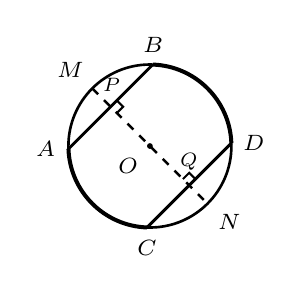
\begin{tikzpicture}[scale=0.75, every node/.style={font=\footnotesize, text=black}]
      \coordinate (O) at (1.7,1.45);
      \draw[black, line width=0.95pt] (O) circle (1.38);
      \coordinate (M) at ($(O)+(135:1.38)$);
      \coordinate (N) at ($(O)+(-45:1.38)$);
      \coordinate (A) at ($(O)+(182:1.38)$);
      \coordinate (B) at ($(O)+(88:1.38)$);
      \coordinate (C) at ($(O)+(-92:1.38)$);
      \coordinate (D) at ($(O)+(2:1.38)$);
      \coordinate (P) at ($(M)!(A)!(N)$);
      \coordinate (Q) at ($(M)!(C)!(N)$);
      \draw[black, line width=0.90pt, dashed] (M)--(N);
      \draw[black, line width=1.05pt] (A)--(B) (C)--(D);
      \draw[black, line width=1.45pt] (A) arc (182:268:1.38);
      \draw[black, line width=1.45pt] (D) arc (2:88:1.38);
      \draw[black, line width=0.75pt] ($(P)+(-45:0.15)$)--($(P)+(-45:0.15)+(45:0.15)$)--($(P)+(45:0.15)$);
      \draw[black, line width=0.75pt] ($(Q)+(135:0.15)$)--($(Q)+(135:0.15)+(45:0.15)$)--($(Q)+(45:0.15)$);
      \fill[black] (O) circle (1.4pt) node[below left=1pt] {$O$};
      \node[above left=0.5pt] at (M) {$M$};
      \node[below right=0.5pt] at (N) {$N$};
      \node[left=1pt] at (A) {$A$};
      \node[above=1pt] at (B) {$B$};
      \node[below=1pt] at (C) {$C$};
      \node[right=1pt] at (D) {$D$};
      \node[above=2pt] at (P) {\scriptsize $P$};
      \node[above=2pt] at (Q) {\scriptsize $Q$};
    \end{tikzpicture}
  \end{minipage}
\end{tcolorbox}

\begin{tcolorbox}[enhanced, sharp corners, colback=panelgray, colframe=black, boxrule=0.90pt, top=4pt, bottom=4pt, left=6pt, right=6pt, after skip=5pt]
  \begin{minipage}[c]{12.8cm}
    \textbf{គំរូទី២ (លំហាត់ទី៤ ទំ.២០៤ — គណនាប្រវែងអង្កត់ធ្នូស្មើចម្ងាយពីផ្ចិត)៖}\\
    ក្នុងរង្វង់ផ្ចិត $O$ គេមានចម្ងាយកែង $OQ = OR$ ($OQ\perp AB, OR\perp CD$) ហើយ $AB = 6x + 14$ និង $CD = -4x + 4$ ។ គណនាប្រវែងអង្កត់ធ្នូ $AB$ និង $CD$ ។\\[2pt]
    $\bullet$ ដោយ $OQ = OR$ តាមហេតុផល \cnum{5} គេបានអង្កត់ធ្នូទាំងពីរប៉ុនគ្នា ($AB = CD$)៖\\
    \hspace*{0.4cm}$6x + 14 =$ \dotline{2.2cm} $\implies 6x + 4x =$ \dotline{1.8cm} $\implies 10x =$ \dotline{1.3cm} $\implies x =$ \dotline{1.1cm} ។\\[2pt]
    $\bullet$ ជំនួសតម្លៃ $x$ រកប្រវែងអង្កត់ធ្នូ និងផ្ទៀងផ្ទាត់ភាពវិជ្ជមាន៖\\
    \hspace*{0.4cm}$AB = 6($\dotline{0.9cm}$) + 14 =$ \dotline{1.2cm} \quad និង \quad $CD = -4($\dotline{0.9cm}$) + 4 =$ \dotline{1.2cm} ($>0$ ផ្ទៀងផ្ទាត់!) ។
  \end{minipage}\hfill
  \begin{minipage}[c]{5.4cm}
    \centering
    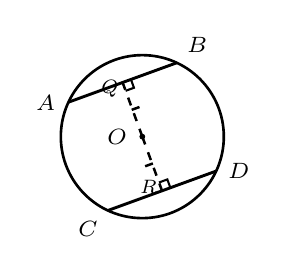
\begin{tikzpicture}[scale=0.75, every node/.style={font=\footnotesize, text=black}]
      \coordinate (O) at (1.7,1.45);
      \draw[black, line width=0.95pt] (O) circle (1.38);
      \coordinate (A) at ($(O)+(155:1.38)$);
      \coordinate (B) at ($(O)+(65:1.38)$);
      \coordinate (C) at ($(O)+(-115:1.38)$);
      \coordinate (D) at ($(O)+(-25:1.38)$);
      \coordinate (Q) at ($(A)!0.5!(B)$);
      \coordinate (R) at ($(C)!0.5!(D)$);
      \draw[black, line width=1.05pt] (A)--(B) (C)--(D);
      \draw[black, line width=0.90pt, dashed, tk1] (O)--(Q);
      \draw[black, line width=0.90pt, dashed, tk1] (O)--(R);
      \draw[black, line width=0.75pt] ($(Q)+(-70:0.15)$)--($(Q)+(-70:0.15)+(20:0.15)$)--($(Q)+(20:0.15)$);
      \draw[black, line width=0.75pt] ($(R)+(110:0.15)$)--($(R)+(110:0.15)+(20:0.15)$)--($(R)+(20:0.15)$);
      \fill[black] (O) circle (1.4pt) node[left=2pt] {$O$};
      \node[left=1pt] at (A) {$A$};
      \node[above right=0.5pt] at (B) {$B$};
      \node[below left=0.5pt] at (C) {$C$};
      \node[right=1pt] at (D) {$D$};
      \node at ($(Q)+(205:0.24)$) {\scriptsize $Q$};
      \node at ($(R)+(165:0.24)$) {\scriptsize $R$};
    \end{tikzpicture}
  \end{minipage}
\end{tcolorbox}

% -------------------- ផ្នែកទី៥៖ E5 EVALUATE --------------------
\secbar{ផ្នែកទី៥ ៖ លំហាត់ប្រតិបត្តិដោយខ្លួនឯង និងតេស្តវាយតម្លៃរហ័ស \enbf{(E5 — Evaluate)}}{\en{10} នាទី (ទំ.២០៣)}

\noindent
\begin{minipage}[t]{11.3cm}
  \begin{tcolorbox}[enhanced, sharp corners, colback=white, colframe=black, boxrule=0.90pt, top=4pt, bottom=4pt, left=5pt, right=5pt, equal height group=e5c4]
    \textbf{១. អនុវត្ត «ប្រតិបត្តិ» (សៀវភៅគោល ទំ.២០៣)៖}\\
    គេឱ្យរង្វង់មួយមានផ្ចិត $O$ និងអង្កត់ផ្ចិត $AD$ ហើយ $AB \parallel CD$ ដូចរូប ។ ចូរបង្ហាញថាអង្កត់ធ្នូ $AB = CD$ ។\\[2pt]
    \begin{minipage}[c]{6.4cm}
      $\bullet$ ដោយអង្កត់ធ្នូ $AB \parallel CD$ (សម្មតិកម្ម)\\
      \hspace*{0.25cm}$\implies$ ធ្នូ $\arc{AC} =$ \dotline{1.3cm} (តាម \dotline{0.9cm}) ។\\[2pt]
      $\bullet$ ដោយ $AD$ ជាអង្កត់ផ្ចិត នោះកន្លះរង្វង់ទាំងពីរស្មើគ្នា៖\\
      \hspace*{0.25cm}$\arc{ACD} = \arc{ABD} =$ \dotline{1.3cm} ។\\[2pt]
      $\bullet$ ដកធ្នូស្មើគ្នា៖ $\arc{CD} = \arc{ACD} - \arc{AC}$\\
      \hspace*{0.25cm}$= \arc{ABD} -$ \dotline{1.1cm} $=$ \dotline{1.1cm} ។\\[2pt]
      $\bullet$ ដូចនេះ អង្កត់ធ្នូ $AB =$ \dotline{1.4cm} ។
    \end{minipage}\hfill
    \begin{minipage}[c]{4.1cm}
      \centering
      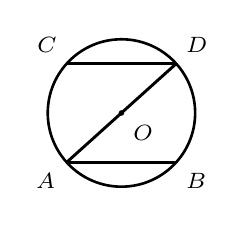
\begin{tikzpicture}[scale=0.72, every node/.style={font=\footnotesize, text=black}]
        \coordinate (O) at (1.5,1.4);
        \draw[black, line width=0.95pt] (O) circle (1.30);
        \coordinate (A) at ($(O)+(222:1.30)$);
        \coordinate (B) at ($(O)+(-42:1.30)$);
        \coordinate (C) at ($(O)+(138:1.30)$);
        \coordinate (D) at ($(O)+(42:1.30)$);
        \draw[black, line width=1.05pt] (A)--(D);
        \draw[black, line width=1.05pt] (A)--(B) (C)--(D);
        \fill[black] (O) circle (1.4pt) node[below right=1pt] {$O$};
        \node[below left=0.5pt] at (A) {$A$};
        \node[below right=0.5pt] at (B) {$B$};
        \node[above left=0.5pt] at (C) {$C$};
        \node[above right=0.5pt] at (D) {$D$};
      \end{tikzpicture}
    \end{minipage}
  \end{tcolorbox}
\end{minipage}\hfill
\begin{minipage}[t]{7.4cm}
  \begin{tcolorbox}[enhanced, sharp corners, colback=white, colframe=black, boxrule=0.90pt, top=4pt, bottom=4pt, left=5pt, right=5pt, equal height group=e5c4]
    \textbf{២. បិទបេសកកម្ម E1 (លូបេតុងមូល)៖}\\
    $HD = \sqrt{5^2 - 3^2} =$ \dotline{0.9cm}$\unit{dm} \implies$ ទទឹងផ្ទៃទឹក $CD = 2HD =$ \dotline{1.1cm}$\unit{dm}$ ។\\[4pt]
    \textbf{៣. តេស្តរហ័ស (\en{Exit Check})៖}\\
    ក្នុងរង្វង់ $C(O, 10\unit{cm})$ អង្កត់ធ្នូ $MN$ ស្ថិតនៅចម្ងាយកែង $OH = 6\unit{cm}$ ពីផ្ចិត $O$ ។ តើប្រវែងអង្កត់ធ្នូ $MN$ ស្មើប៉ុន្មាន?\\[3pt]
    \chk\ \textbf{A.} $8\unit{cm}$ \hspace{1.1cm} \chk\ \textbf{B.} $12\unit{cm}$\\[2.5pt]
    \chk\ \textbf{C.} $16\unit{cm}$ \hspace{0.95cm} \chk\ \textbf{D.} $20\unit{cm}$\\[4pt]
    \textbf{ការគណនា៖} $HN = \sqrt{10^2 - 6^2} =$ \dotline{1.2cm}$\unit{cm}$\\
    នាំឱ្យប្រវែងពេញ $MN = 2HN =$ \dotline{1.4cm}$\unit{cm}$ ។
  \end{tcolorbox}
\end{minipage}

% -------------------- ផ្នែកទី៦៖ កិច្ចការផ្ទះ --------------------
\vspace{6pt}
\begin{tcolorbox}[enhanced, sharp corners, colback=panelgray, colframe=black, boxrule=0.95pt, top=4.5pt, bottom=4.5pt, left=6pt, right=6pt]
  \begin{minipage}[c]{14.2cm}
    {\muol\fontsize{9.0pt}{13.5pt}\selectfont ផ្នែកទី៦ ៖ កិច្ចការផ្ទះ និងបណ្ដាំផ្ញើ (សៀវភៅសិក្សាគោល ទំព័រ ២០៤ — ធ្វើក្នុងសៀវភៅលំហាត់)}\\[2.5pt]
    $\bullet$ \textbf{លំហាត់ទី៩ (ទំ.២០៤)៖} គេមានរង្វង់ $C(O, r)$ និងចំណុច $P$ នៅក្នុងរង្វង់នេះ ($P\ne O$) ។ ស្រាយបញ្ជាក់ថាក្នុងចំណោមអង្កត់ធ្នូទាំងអស់ដែលកាត់តាមចំណុច $P$ អង្កត់ធ្នូដែលកែងនឹង $OP$ មានប្រវែងខ្លីជាងគេ (ណែនាំ៖ ប្រៀបធៀបចម្ងាយកែង $OH \le OP$ តាមពីតាករ) ។\\[2.5pt]
    $\bullet$ \textbf{លំហាត់ទី១០ ក (ទំ.២០៤)៖} អង្កត់ធ្នូ $AB$ និង $CD$ ($AB>CD$) កាត់គ្នាត្រង់ $K$ នៅក្រៅរង្វង់ផ្ចិត $O$ ។ $H$ និង $P$ ជាចំណុចកណ្ដាលនៃ $AB$ និង $CD$ ។ ស្រាយបញ្ជាក់ថាចំណុចកណ្ដាលនៃ $OK$ ស្មើចម្ងាយពី $O, K, P, H$ និងអានមុន \textbf{មេរៀនទី១៦ ៖ បន្ទាត់ និងរង្វង់} (ទំ.២០៥) ។
  \end{minipage}\hfill
  \begin{minipage}[c]{4.1cm}
    \centering
    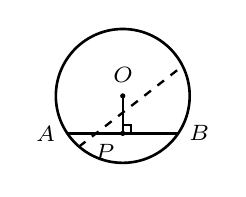
\begin{tikzpicture}[scale=0.68, every node/.style={font=\footnotesize, text=black}]
      \coordinate (O) at (1.5,1.45);
      \draw[black, line width=0.95pt] (O) circle (1.25);
      \coordinate (P) at (1.5,0.75);
      \coordinate (A) at (0.46,0.75);
      \coordinate (B) at (2.54,0.75);
      \coordinate (C) at (0.68,0.50);
      \coordinate (D) at (2.58,1.98);
      \draw[black, line width=1.05pt] (A)--(B);
      \draw[black, line width=0.85pt, dashed] (C)--(D);
      \draw[black, line width=0.90pt] (O)--(P);
      \draw[black, line width=0.7pt] ($(P)+(0,0.16)$)--($(P)+(0.16,0.16)$)--($(P)+(0.16,0)$);
      \fill[black] (O) circle (1.4pt) node[above=1pt] {$O$};
      \fill[black] (P) circle (1.4pt) node[below left=0.5pt] {$P$};
      \node[left=0.5pt] at (A) {$A$};
      \node[right=0.5pt] at (B) {$B$};
    \end{tikzpicture}
  \end{minipage}
\end{tcolorbox}

\end{document}
